\graphicspath{{content/chapters/4_specification/figures/}}
\chapter{Specification}
\label{chp:specification}

The 

\section{Dataset Exploration}
\label{sec:dataset_exploration}

A key aspect of defining the system specifications is understanding the dataset being used. This project utilizes an open-source dataset titled \textit{"Noisy speech database for training speech enhancement algorithms and TTS models"}, available through the \textit{DataShare} repository at the University of Edinburgh~\cite{edinburghdataset}. The dataset is licensed under the Creative Commons Attribution 4.0 International License~\cite{ccby4}.

\url{https://datashare.ed.ac.uk/handle/10283/2791}

\begin{figure}[H]
    \centering
    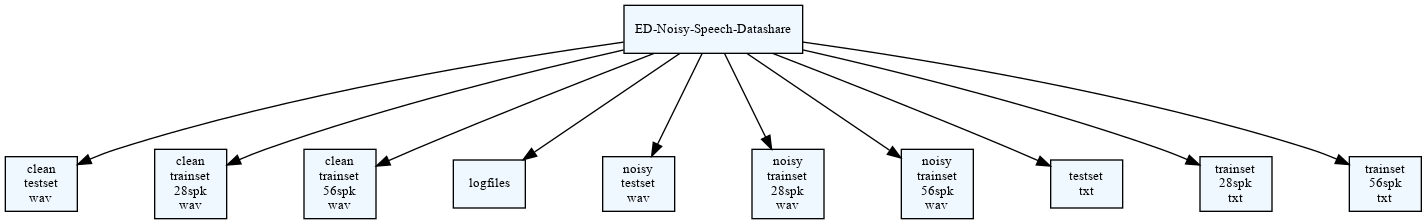
\includegraphics[width=1.0 \textwidth]{dataset_structure.png}
    \caption{Dataset Tree Structure}
    \label{fig:dataset_structure}
\end{figure}

The dataset contains three main subsets: a test set, a 28-speaker training set, and a 56-speaker training set. Each subset consists of separate folders containing transcripts, clean speech, and noisy speech. The files within each folder are aligned in order, meaning that the same index in each folder corresponds to the same audio sample, ensuring parallelism between clean and noisy data. However, it is important to note that the file numbering is not continuous and includes gaps in the sequence.

\begin{figure}[H]
    \centering
    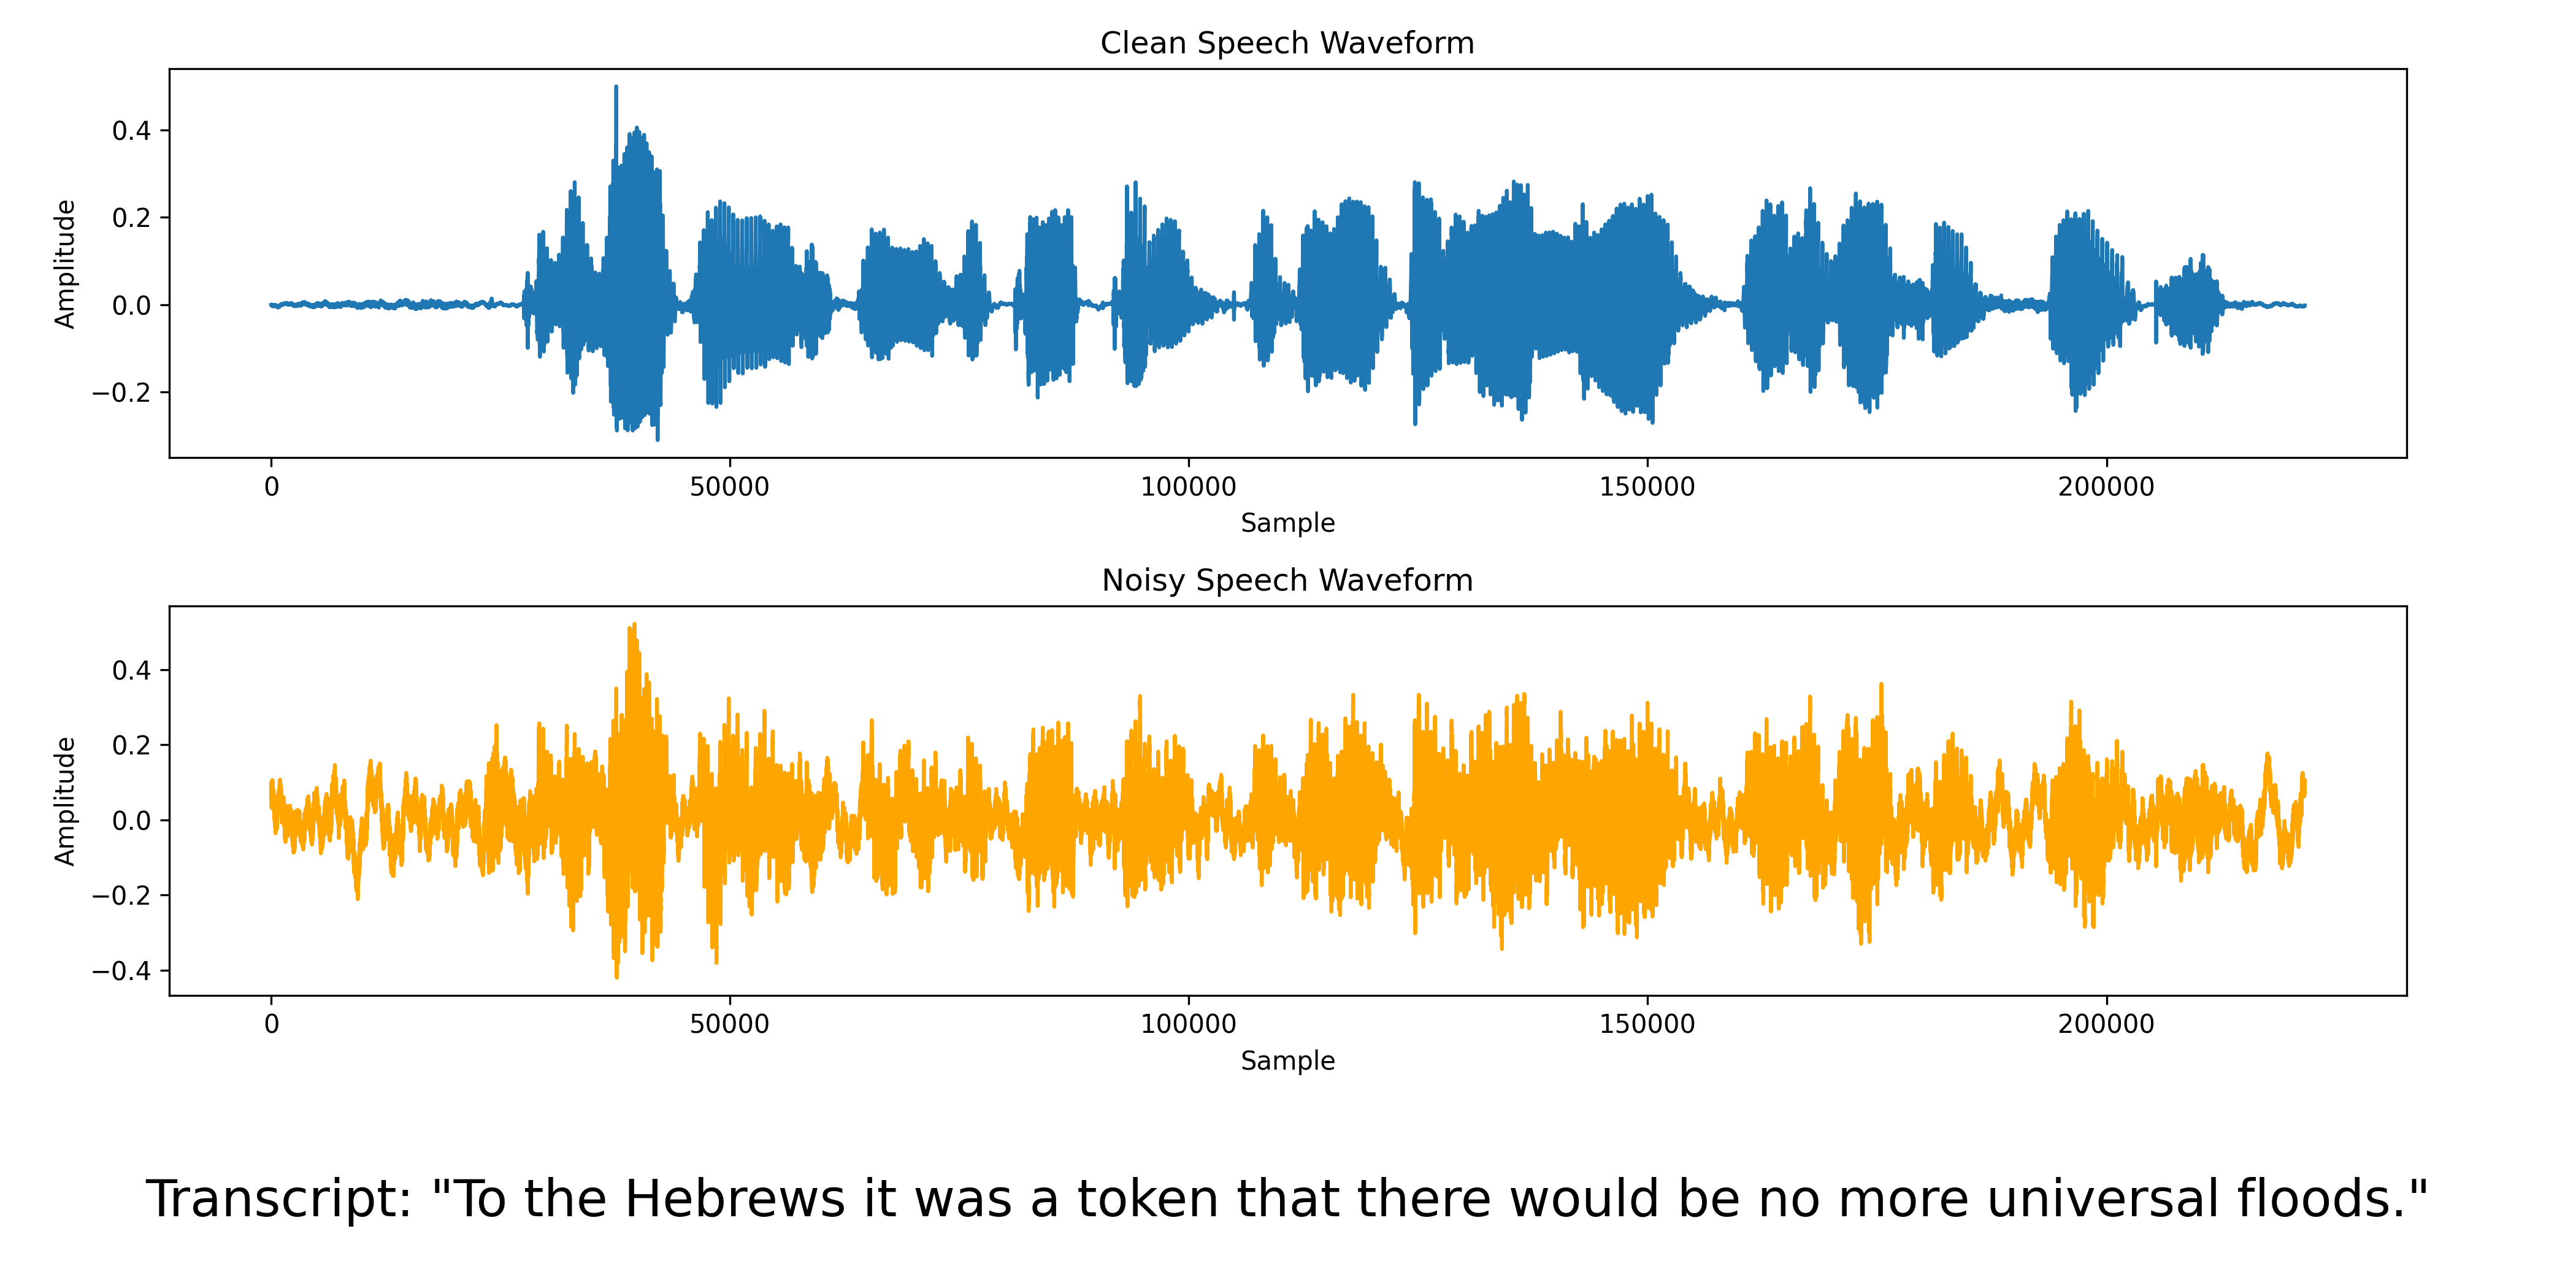
\includegraphics[width=0.8\textwidth]{sample_waveform_and_transcript.png}
    \caption{Example of a Clean, Noisy Speech Sample and its Transcript}
    \label{fig:sample_waveform_and_transcript}
\end{figure}

All speech files are in \texttt{.wav} format and are sampled at 48~kHz. The audio clips vary in length, which is a key consideration in the system's design, especially for batching and model input formatting. The dataset contains no corrupted files, and the total download size, as recorded by the \texttt{wget} log, was approximately 15~GB.

\section{System Requirements}
\label{sec:system_requirements}

Due to the nature of the project, which involves training a neural network model, the system requirements are primarily focused on the hardware and software specifications necessary for efficient computation. The project was developed and executed remotely on the University of Malta Interfacing Lab computers, which are accessible to students via SSH. These remote machines are equipped with NVIDIA GeForce RTX 3060 GPUs, which are suitable for deep learning tasks. However, due to memory constraints, limitations on the number of epochs, batch size, and model architecture were imposed to prevent exceeding resource limits.

The primary development environment for this project was Visual Studio Code (VSCode), enhanced with GitHub Copilot, which assisted with both syntactic and semantic aspects of coding. Initial development was carried out using individual Jupyter notebooks, which facilitated easy testing and debugging of isolated components. These notebooks were later consolidated into a single Python application for deployment and future extension.

The final application was designed with a modular architecture, consisting of separate files for data preprocessing, model training, and evaluation. This structure improves maintainability and supports future updates or integration with other systems.

The output of the system is a trained deep learning model saved as a model path file. This file can be used for inference on new audio samples and is compatible with widely used deep learning frameworks such as TensorFlow or PyTorch. The model is designed to be transferable, allowing it to be deployed on different machines or embedded boards to replicate the speech enhancement process in real-world applications.
